\section{A J-Integral for pressurized cracks in a phase-field setting}\label{sec:j_integral}

%In the field of Fracture Mechanics, a very important tool for assessing the phenomena of propagation is the so-called J-Integral \cite{rice1968mathematical, rice1968path, rice1973some}. {\color{purple}This contour integral, in its basic form, is path independent and provides a simple way to retrieve the energy release rate of a given mechanical configuration.} When a phase-field description of fracture is used, in most of the time, an explicit computation of the energy release rate is not necessary, as the balance between elastic and fracture energy is enforced by the variational principle. {\color{purple}Nevertheless, with certain modifications, the J-Integral can also be applied in the regularized setting as a verification tool, as in \cite{hossain2014effective, kumar2020revisiting}.}

%With respect to the novel model described in Section \ref{sec:model}, it is important to assess how well it satisfies Griffith's law for finite values of $\ell$ and whether it converges as $\ell \rightarrow 0$. For this purpose, it is necessary to extract the instantaneous energy release rate (here denoted as $G$) of pressurized cracks in a phase-field context. 

This Section presents a modified J-integral, capable of retrieving $G$ in the case of pressurized cracks in a phase-field for fracture setting. The resulting integral is then re-cast into a domain-independent form that is more amenable to finite-element calculations.  
 

%{\color{purple}This J-Integral is re-cast in the domain form, which has a few advantages compared to the contour form. First, the implementation is simpler when used in the finite element context, as it only needs integration over elements, allowing standard quadrature rules to be used. Second, it also retains improved accuracy, since it does not require interpolation of quantities outside of quadrature points.} 

%The first use of the J-Integral in the context of phase-field fracture dates back to the work of Hakim and Karma \cite{hakim2009laws}, who used it to study the fracture model proposed in \cite{karma2001phase}. Later, in \cite{sicsic2013gradient} and \cite{ballarini2016closed} the concept was applied to the phase-field model based on the regularization of the variational approach to fracture of Francfort and Marigo \cite{francfort1998revisiting}. In these works, the expression of the J-Integral, which works in general, for traction-free cracks is,

A common form of the J-integral, derived for phase-field fracture and applicable to traction-free cracks is given by \cite{sicsic2013gradient,ballarini2016closed} 
\begin{equation}
    J = \textbf{r} \cdot \int\limits_{\zeta} \biggl( \psi(\bs\epsilon, d)\mathbb{I} - \nabla \textbf{u}^T\bs \sigma-\nabla d \otimes \bs\omega \biggr) \textbf{n}\text{ds}, 
\end{equation}
where $\psi(\bs\epsilon, d)$ is given by equation \eqref{PF general form}. In the above, the vector $\textbf{r}$ denotes the crack propagation direction, $\zeta$ is a closed path around the crack tip, $\mathbb{I}$ is the second-order identity tensor, $\textbf{n}$ is the normal to the closed path $\zeta$ and $\bs\omega = \partial \psi/\partial \nabla d = (G_c\ell/c_0)\nabla d$. Compared to the original form of the J-integral proposed by Rice~\cite{rice1968mathematical,rice1968path}, this expression contains additional terms to account for the phase-field parameter $d$. 

Importantly,  Sicsic and Marigo \cite{sicsic2013gradient} show that, under certain conditions, the standard form of the J-integral widely employed for sharp cracks, viz.
\begin{equation}
    J = \textbf{r} \cdot \int\limits_{\zeta} \biggl( \psi_e(\bs\epsilon, d)\mathbb{I} - \nabla \textbf{u}^T\bs \sigma\biggr) \textbf{n}\text{ds},
\end{equation}
 can be used in a regularized phase-field setting. These conditions are:

\begin{enumerate}[start=1,label={\bfseries H\arabic*}]
    \item \label{itm:hyp1}: The regularization length is sufficiently small, so that a separation of scales between the solution in the damage band and the outer solution can be achieved;

    \item \label{itm:hyp2}: The path $\zeta$ intersects the crack plane at a ninety-degree angle;

    \item \label{itm:hyp3}: The path $\zeta$ intersects the crack plane sufficiently far from the crack tip, so that the damage field only varies in a direction perpendicular to the crack plane.   
\end{enumerate}

\noindent In what follows, these same conditions are assumed, as they facilitate a simpler derivation of a modified J-Integral capable of retrieving the energy release rate even in the presence of pressure loads on the crack faces. The main result of this section can then be stated in the following way.

% \begin{figure}[h]
%     \centering
%     \begin{tikzpicture}
%         \node {\pgfimage[interpolate=false,width=.4\textwidth]{images/theory_part/potato_crack.png}};
%         \draw (-0.1\textwidth,-0.1\textwidth) node {\LARGE$\Omega$};
%         \draw (0.03\textwidth,0.03\textwidth) node {\LARGE\color{blue}$p$};
%         \draw (0.075\textwidth,-0.05\textwidth) node {\LARGE$\Gamma$};
%         \draw (0.16\textwidth,0.16\textwidth) node {\LARGE$\textbf{t}$};
%     \end{tikzpicture}
%     \caption{Generic body containing cracks loaded in pressure.}
%     \label{fig:potato}
% \end{figure}

\begin{figure}[ht]
% \centering
\begin{subfigure}{.49\textwidth}
  \centering
  % \begin{tikzpicture}
  %       \node {\pgfimage[interpolate=false,width=.8\textwidth]{images/theory_part/j_integral.png}};
  %       \draw (-0.18\textwidth,-0.1\textwidth) node {\LARGE$\Lambda$};
  % \end{tikzpicture}
  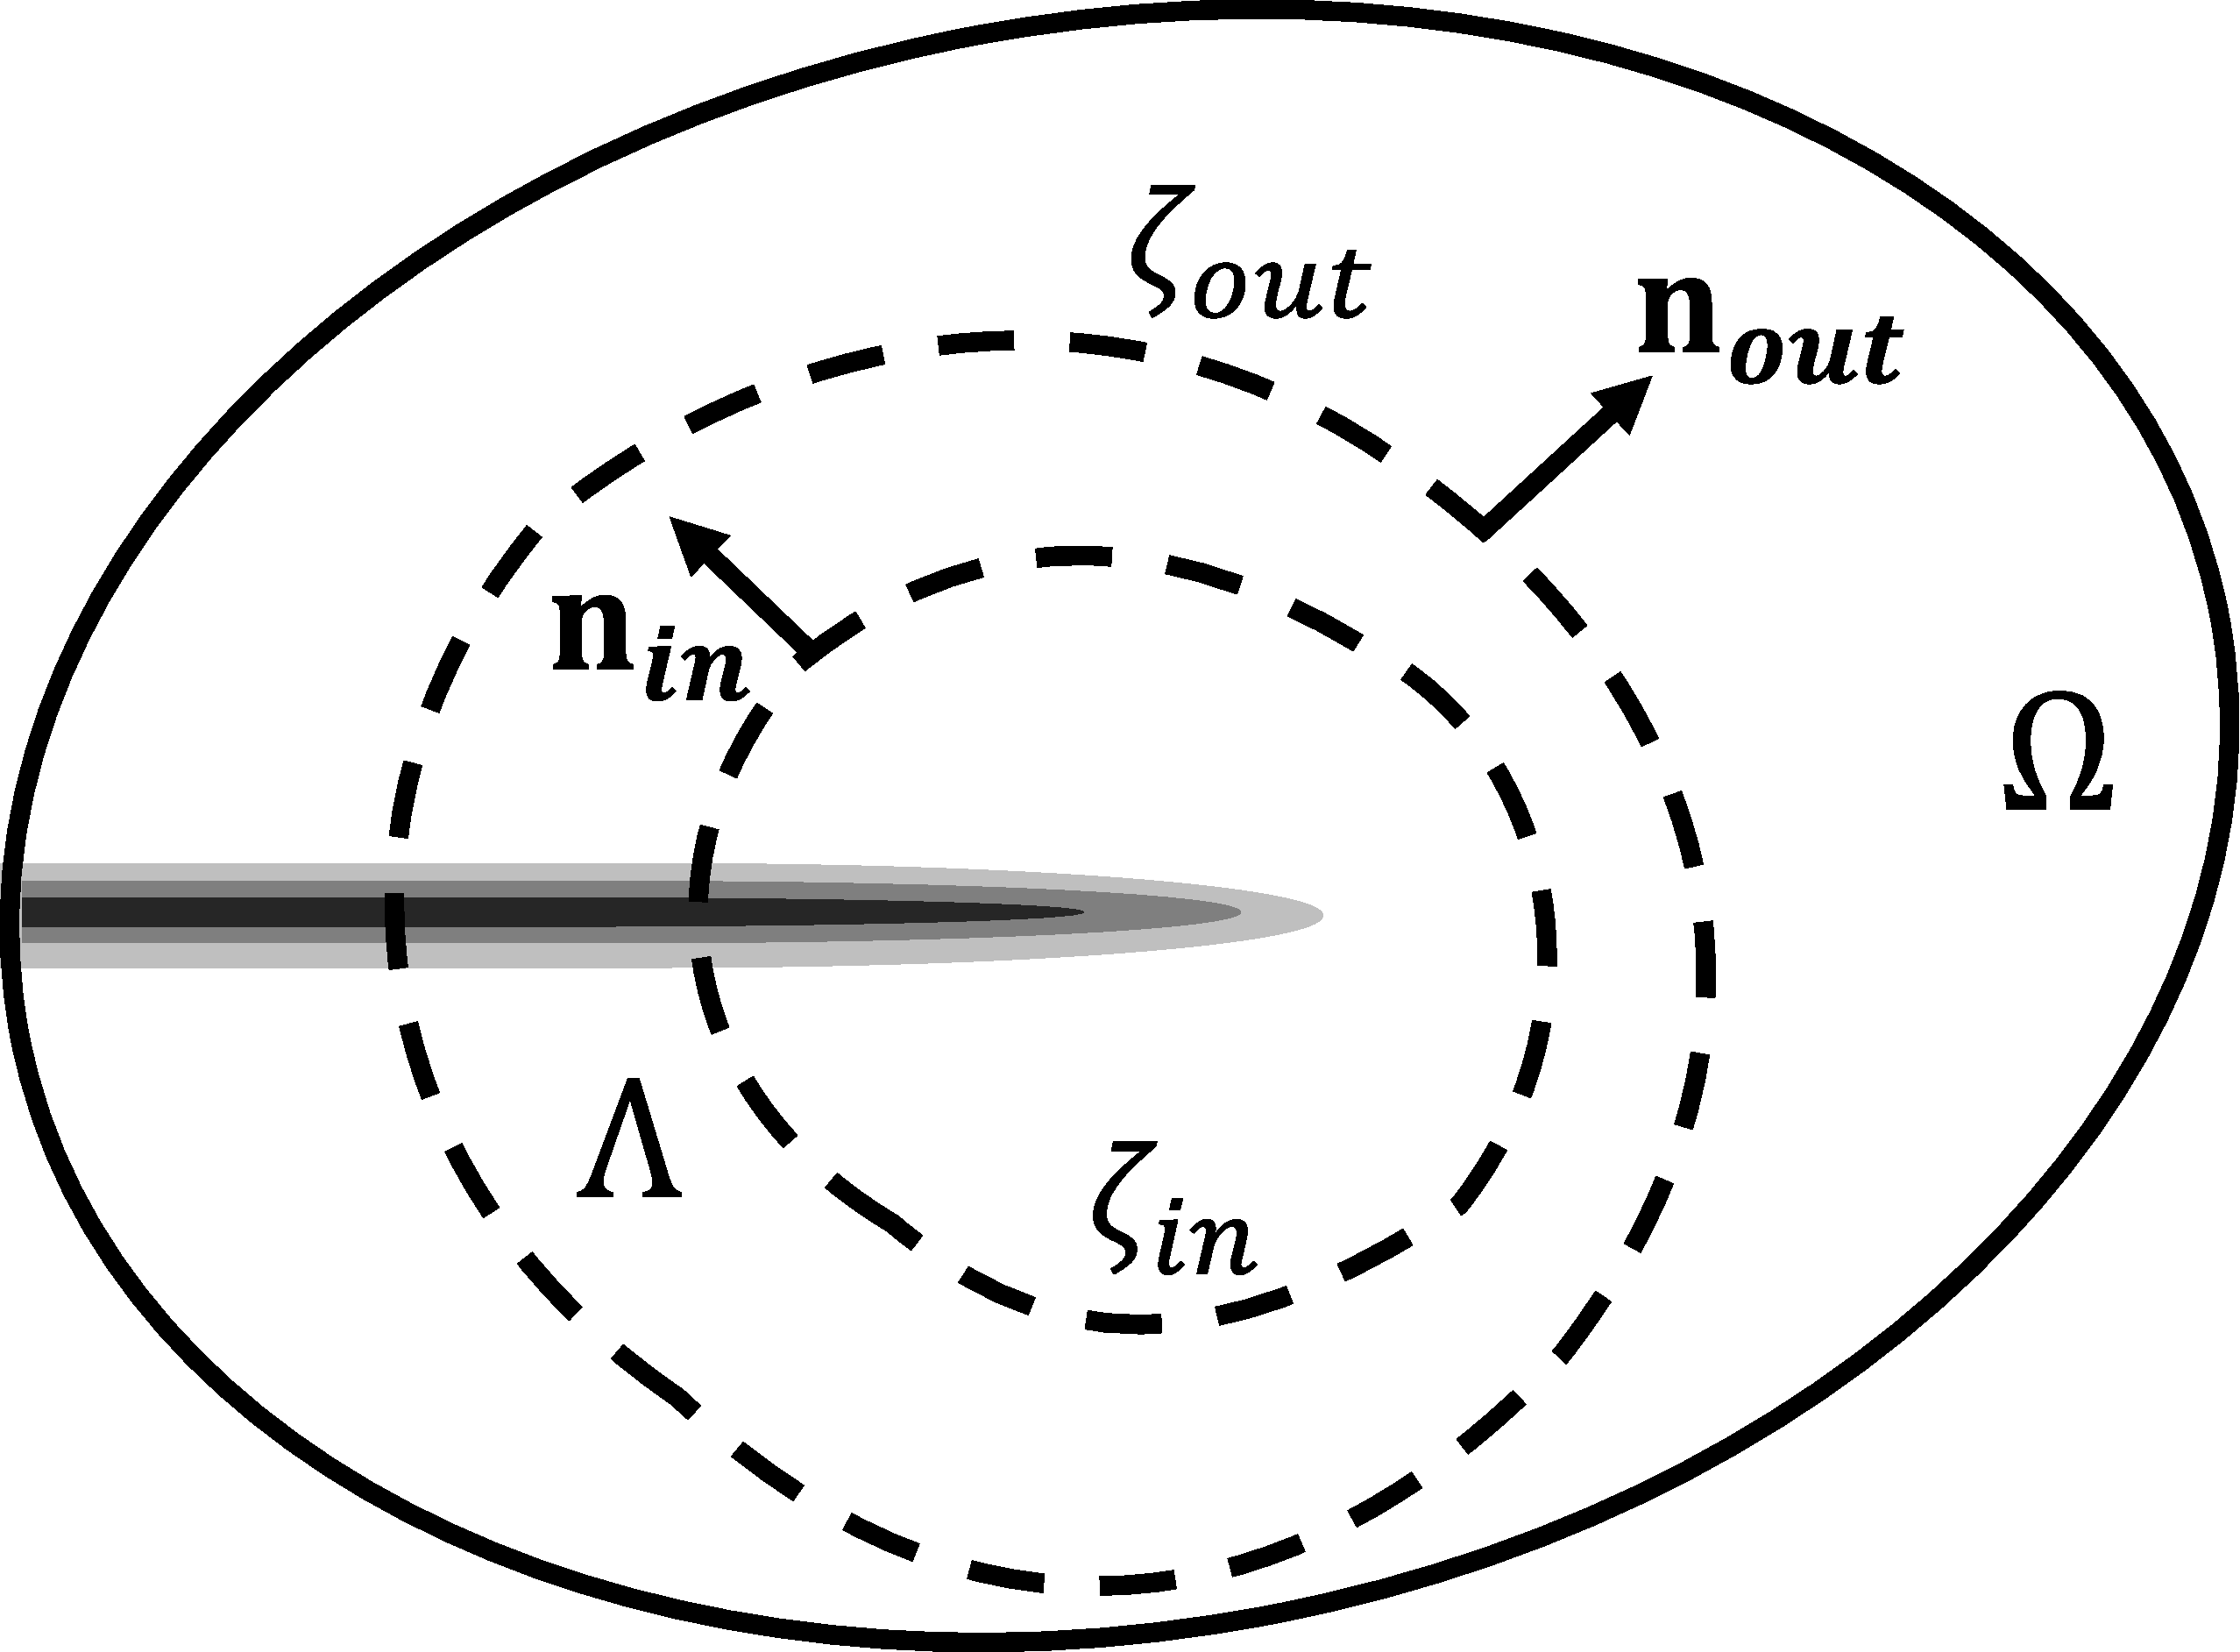
\includegraphics[width=0.8\linewidth]{images/theory_part/j_integral_bw.pdf}
  \bigskip
  \bigskip
  \caption{}
  \label{fig:j_integral}
\end{subfigure}%
\begin{subfigure}{.49\textwidth}
  \centering
  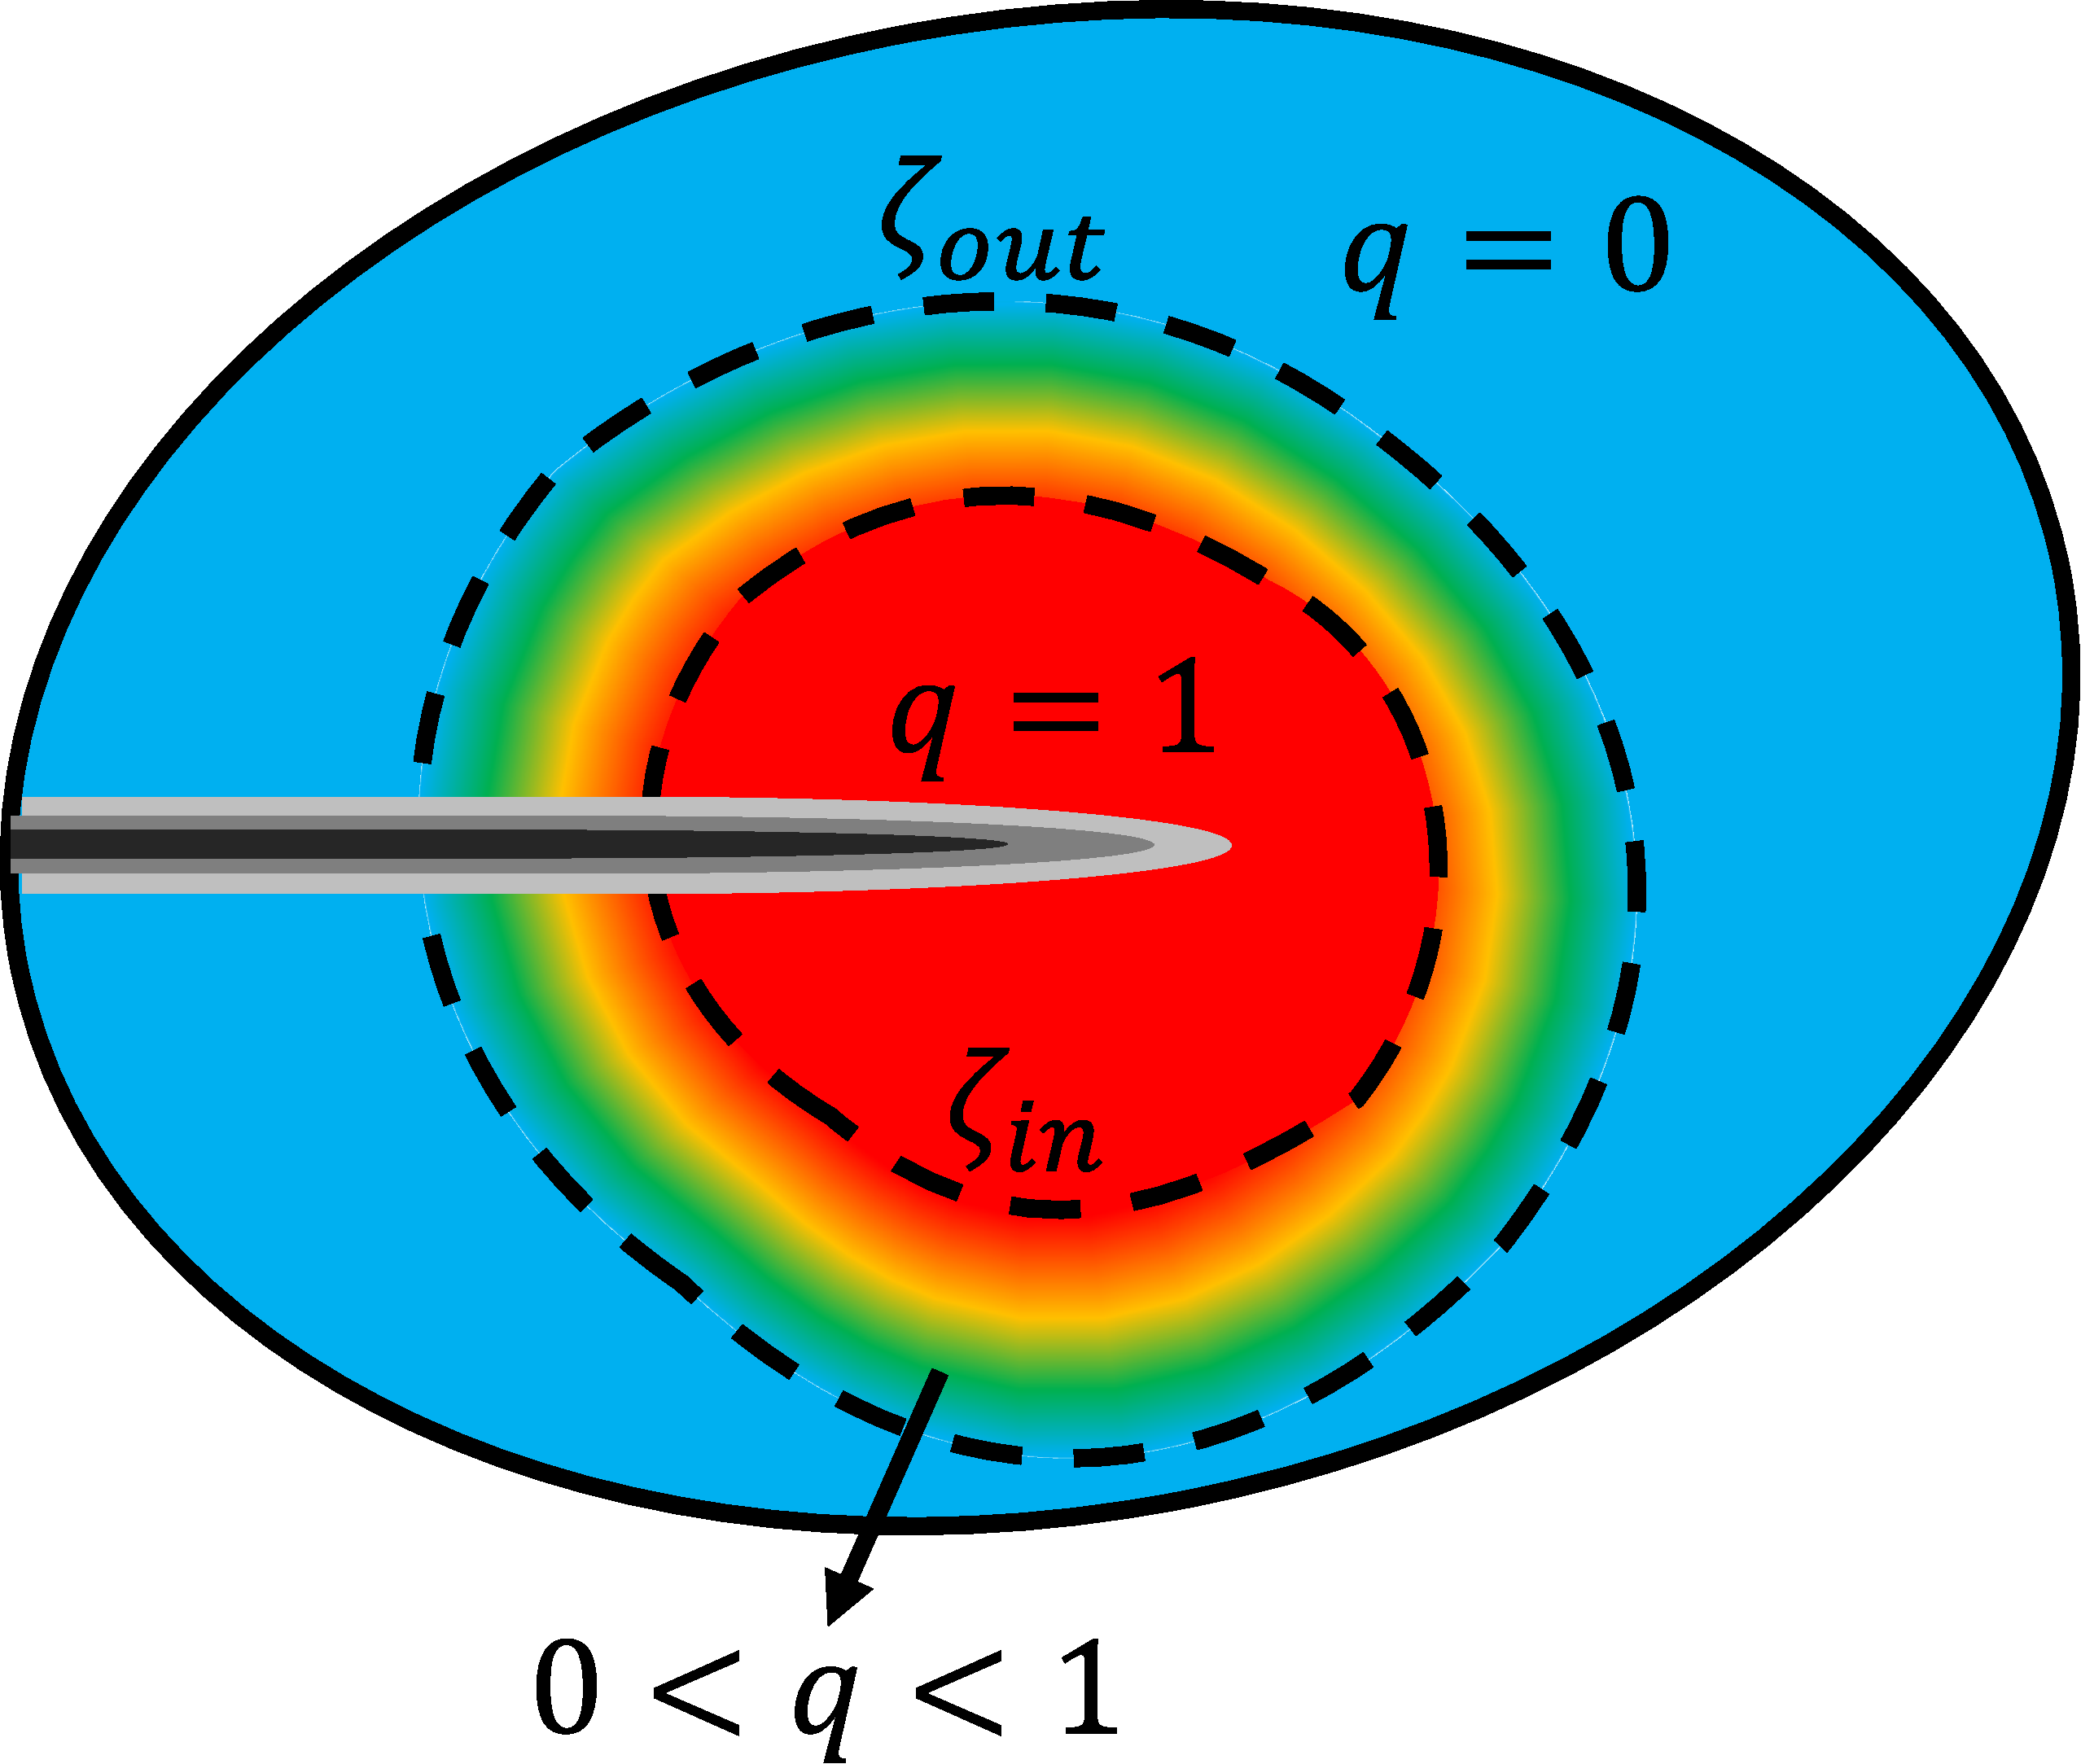
\includegraphics[width=0.8\linewidth]{images/theory_part/j_integral_bw_q.pdf}
  \caption{}
  \label{fig:j_integral_q}
\end{subfigure}%
  \caption{(a) The contour paths $\zeta_{in}$ and $\zeta_{out}$ and subdomain $\Lambda$, in the vicinity of a regularized crack.; (b) Color contour plot indicating the assumed variation in the function $q$.  } 
  \label{fig:j_integral_pics}
\end{figure}

% \begin{figure}[ht]
% % \centering
% \begin{subfigure}{.49\textwidth}
%   \centering
%   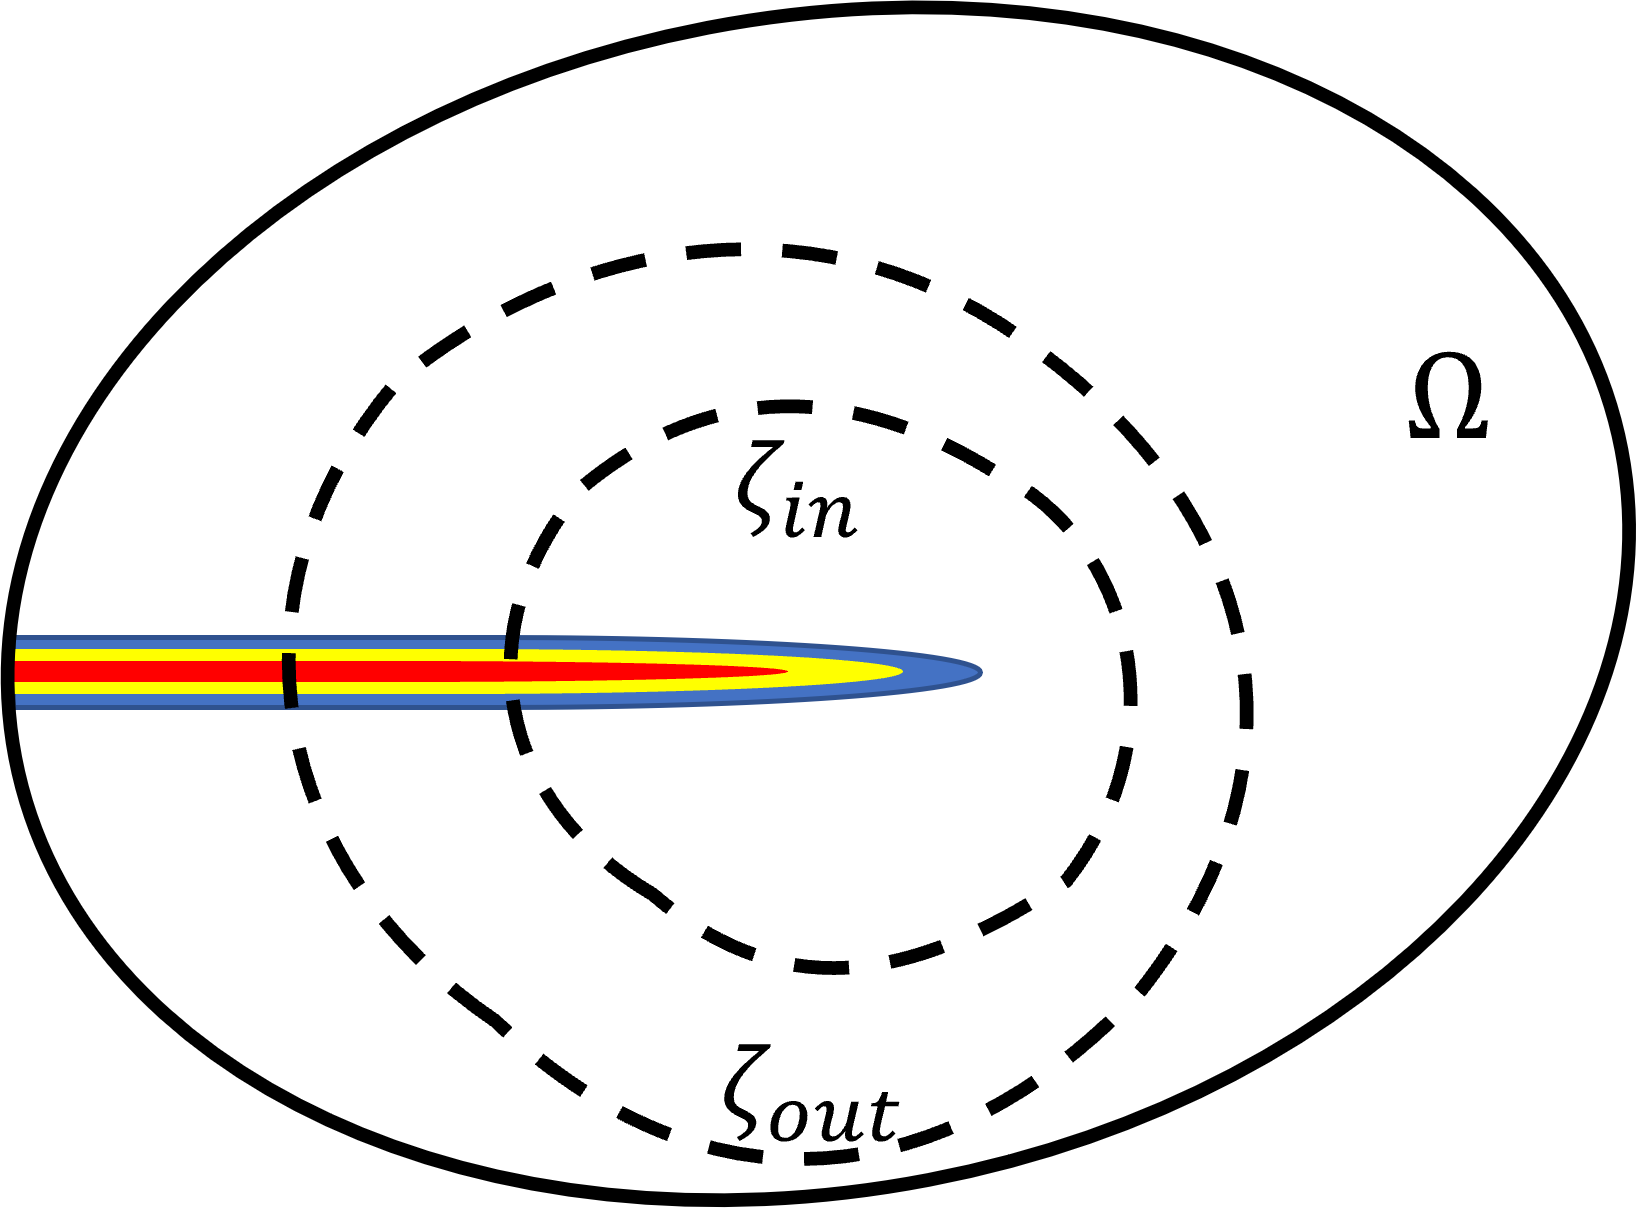
\includegraphics[width=0.8\linewidth]{images/theory_part/j_integral.pdf}
%   \bigskip
%   \bigskip
%   \caption{}
%   \label{fig:j_integral}
% \end{subfigure}%
% \begin{subfigure}{.49\textwidth}
%   \centering
%   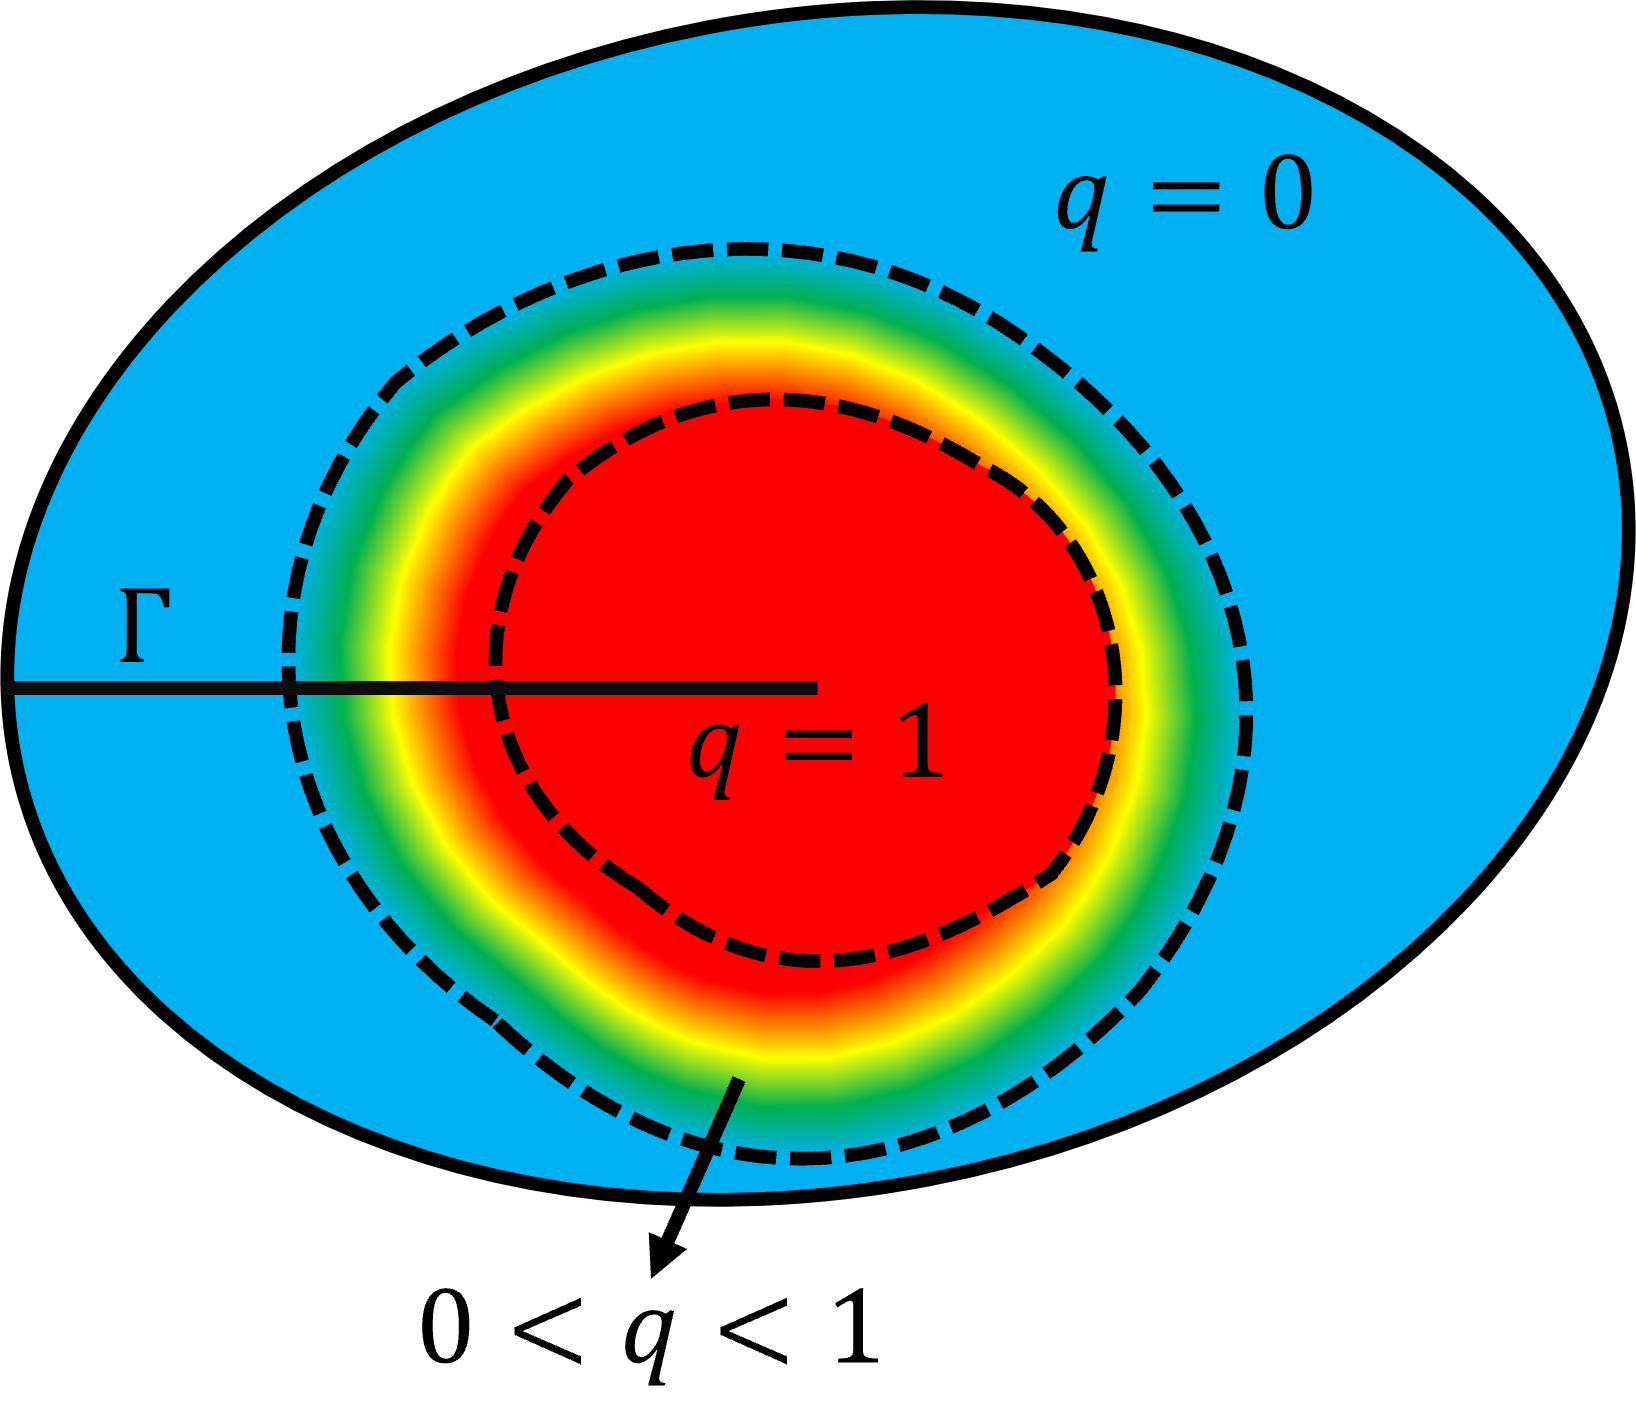
\includegraphics[width=0.8\linewidth]{images/theory_part/j_integral_q.pdf}
%   \caption{}
%   \label{fig:j_integral_q}
% \end{subfigure}%
%   \caption{(a) Description of paths $\zeta_{in}$ and $\zeta_{out}$.; (b) Description of the function $q$. ADD $\Lambda$ TO FIRST FIGURE.} 
%   \label{fig:j_integral_pics}
% \end{figure}

\medskip

\noindent\textbf{Claim}: Consider a domain $\Omega \in \mathbb{R}^2$ with a straight phase-field crack and two closed, non-intersecting paths $\zeta_{in}$ and $\zeta_{out}$ around the crack tip, enclosing an area $\Lambda$ as shown in Figure~\ref{fig:j_integral}. Let $q(x)$ be a sufficently smooth function satisfying $q = 1$ on $\zeta_{in}$ and $q = 0$ on $\zeta_{out}$. Further, assume that $q = 1$ for all points inside $\zeta_{in}$ and $q = 0$ for all points outside $\zeta_{out}$, as shown in Figure \ref{fig:j_integral_q}. Finally, assume that the fracture is loaded by a constant pressure $p$, and that one of the formulations described in Section \ref{sec:model} holds. Then, if conditions \ref{itm:hyp1}, \ref{itm:hyp2} and \ref{itm:hyp3} hold for $\zeta_{in}$ and $\zeta_{out}$, the energy release rate can be approximated by the  integral
\begin{equation}\label{j_integral_theorem}
    J = \textbf{r} \cdot \int\limits_{\Lambda} \biggl( \psi_e(\bs\epsilon, d)\mathbb{I} -p\nabla d\cdot\textbf{u}I'(d)\mathbb{I}  - \nabla \textbf{u}^T\bs \sigma \biggr) \cdot \nabla q\ \text{dA},
\end{equation}

\noindent with an error that vanishes as $\ell \rightarrow 0$. The proof can be established in three steps, as detailed below.

\medskip

\noindent \textbf{Proof:} Define $\textbf{T}_p = \psi_e(\bs\epsilon, d)\mathbb{I} -p\nabla d\cdot\textbf{u}I'(d)\mathbb{I}  - \nabla \textbf{u}^T\bs \sigma$. Using the divergence theorem, one can show that
\begin{equation}
    \int\limits_{\Lambda} \nabla\cdot(q\textbf{T}_p)\text{dA} = \int\limits_{\zeta_{in}\cup\zeta_{out}}q\textbf{T}_p\cdot\textbf{n}\ \text{ds} = 0 - \int\limits_{\zeta_{in}}\textbf{T}_p\cdot\textbf{n}\ \text{ds}, 
\end{equation}
because $q$ vanishes on $\zeta_{out}$ and the normal $\textbf{n}$ to $\zeta_{in}$ points inward to $\Lambda$, as shown in Figure~\ref{fig:j_integral}.  
%sign change in the last term is due to the orientation of the normal $\textbf{n}$. 
Multiplying both sides by the crack direction $\textbf{r}$ and applying the chain rule yields
\begin{equation}\label{first_step}
    -\textbf{r}\cdot\int\limits_{\Lambda} \biggl( \textbf{T}_p\cdot \nabla q + q\nabla \cdot \textbf{T}_p\biggr)\text{dA} =  \textbf{r}\cdot\int\limits_{\zeta_{in}}\textbf{T}_p\cdot\textbf{n}\ \text{ds}, 
\end{equation}
 which completes the first step of the proof. 
 
 The second step consists of showing that the term $R = \textbf{r}\cdot\int\limits_{\Lambda} q\nabla \cdot \textbf{T}_p\ \text{dA}$ is zero. Expanding the expression for $\textbf{T}_p$ and using the chain rule yields
\begin{multline}
    R = \textbf{r}\cdot\int\limits_{\Lambda} q\nabla \cdot \biggl( \psi_e(\bs\epsilon, d)\mathbb{I} -p\nabla d\cdot\textbf{u}I'(d)\mathbb{I}  - \nabla \textbf{u}^T\bs\sigma \biggr)\ \text{dA} = \\
    \int\limits_{\Lambda} q\biggl( \dfrac{\partial \psi_e(\bs\epsilon, d)}{\partial\nabla^s\textbf{u}}\cdot(\nabla(\nabla^s\textbf{u})\textbf{r}) + \dfrac{\partial \psi_e(\bs\epsilon, d)}{\partial d}\nabla d\cdot \textbf{r} 
    - (\nabla \cdot \bs\sigma)\cdot(\nabla\textbf{u}\textbf{r}) - \bs\sigma(\nabla (\nabla\textbf{u})\textbf{r})-p\nabla d\cdot(\nabla \textbf{u}\textbf{r})I'(d) - p\textbf{u}\nabla(I'(d)\nabla d)\textbf{r} \biggr)\ \text{dA}.
\end{multline}
 Re-arranging some terms, one can write,
\begin{equation}
    R = \int\limits_{\Lambda} q\biggl[\biggl( \dfrac{\partial \psi_e(\bs\epsilon, d)}{\partial\nabla^s\textbf{u}}-\bs\sigma\biggr) \cdot(\nabla(\nabla^s\textbf{u})\textbf{r}) 
    -\biggl( \nabla \cdot \bs\sigma - pI'(d) \nabla d \biggr)\cdot (\nabla\textbf{u}\textbf{r})
    + \dfrac{\partial \psi_e(\bs\epsilon, d)}{\partial d}\nabla d\cdot \textbf{r} 
    - p\textbf{u}\nabla(I'(d)\nabla d)\textbf{r} \biggr]\ \text{dA}.
\end{equation}

\noindent For any elastic material, the definition of stress implies $\dfrac{\partial \psi_e(\bs\epsilon, d)}{\partial\nabla^s\textbf{u}}-\bs\sigma = 0$, and due to equation \eqref{u_equation}, $\nabla \cdot \bs\sigma - p \nabla d = 0$, so, the expression above reduces to
\begin{equation}
    R = \int\limits_{\Lambda} q\biggl(\dfrac{\partial \psi_e(\bs\epsilon, d)}{\partial d}\nabla d\cdot \textbf{r} 
    - p\textbf{u}\nabla(I'(d)\nabla d)\textbf{r} \biggr)\ \text{dA}.
\end{equation}
Assuming a separation of scales, the domain $\Lambda$ can be separated into two regions: (i) $\Lambda_{band}$, which consists of the intersection between $\Lambda$ and the support of the damage field representing the crack and (ii) $\Lambda_{outer}$, which denotes the remainder of $\Lambda$, outside of the damage band.  In the asymptotic limit as $\ell\rightarrow 0$, the material in $\Lambda_{outer}$ behaves as purely elastic. Within $\Lambda_{outer}$, one has $d \approx \nabla d \approx 0$, and therefore,  
\begin{equation}
    R_{outer}  = \int\limits_{\Lambda_{outer}} q\biggl(\dfrac{\partial \psi_e(\bs\epsilon, d)}{\partial d}\nabla d\cdot \textbf{r} - p\textbf{u}\nabla(I'(d)\nabla d)\textbf{r} \biggr)\ \text{dA} \approx 0.
\end{equation}
 For the $\Lambda_{band}$ region, by condition \ref{itm:hyp3}, $\nabla d$ is purely perpendicular to the crack direction, so, $\nabla d \cdot \textbf{r} \approx 0$. Therefore,
\begin{equation}
    R_{band} = \int\limits_{\Lambda_{band}} q\biggl(\dfrac{\partial \psi_e(\bs\epsilon, d)}{\partial d}\nabla d\cdot \textbf{r} 
    - p\textbf{u}\nabla(I'(d)\nabla d)\textbf{r} \biggr)\ \text{dA} \approx 0.
\end{equation}


\noindent Since $\Lambda = \Lambda_{band} \cup \Lambda_{outer}$, we must have 

\begin{equation}\label{step2}
    R = R_{outer}+R_{band} \approx 0.
\end{equation}

\noindent This completes the second step. 


The final step of the proof begins by invoking the separation of scales to decompose the contour integral in \eqref{first_step} via
\begin{equation}\label{step3}
    \textbf{r}\cdot\int\limits_{\zeta_{in}}\textbf{T}_p\cdot\textbf{n}\ \text{ds} = \textbf{r}\cdot\biggl(\int\limits_{\zeta^{band}_{in}}\textbf{T}_p\cdot\textbf{n}\ \text{ds} + \int\limits_{\zeta^{outer}_{in}}\textbf{T}_p\cdot\textbf{n}\ \text{ds} \biggr).
\end{equation}
On the $\zeta^{outer}_{in}$ portion of the path, damage effects can be neglected and the integral simplifies to the standard (sharp) J-Integral.  In the case of a uniformly pressurized crack \cite{karlsson1978jintegral}, this gives
% \noindent On the $\zeta^{outer}_{in}$ portion of the path, the second term in the right side of \eqref{step3} reduces to the expression of Rice's J-Integral, which, in the case of a uniformly pressurized crack \cite{karlsson1978jintegral}, evaluates to,
\begin{equation}\label{path_outer}
    \int\limits_{\zeta^{outer}_{in}}\textbf{T}_p\cdot\textbf{n}\ \text{ds} = G - pw,
\end{equation}
where $w$ denotes the crack aperture at the intersection of the crack and the contour $\zeta_{in}$. 

The other portion of the integral can be re-written as
\begin{equation}
    \textbf{r}\cdot \int\limits_{\zeta^{band}_{in}}\textbf{T}_p\cdot\textbf{n}\ \text{ds} = \textbf{r}\cdot\int\limits_{-B}^{B}(\psi_e\mathbb{I}-\nabla \textbf{u}^T\bs\sigma)\cdot\textbf{n}dx - \textbf{r}\cdot\int\limits_{-B}^{B}p(\nabla d\cdot \textbf{u}I'(d))\cdot\textbf{n}dx,
\end{equation}

\noindent where $B$ is the half-length of the damage band and condition \ref{itm:hyp2} is used to transform the integral over $\zeta^{band}_{in}$ to a simple real integral from $-B$ to $B$. Here, both $\textbf{r}$ and $\textbf{n}$ are unit vectors that point in opposite directions, and therefore, $\textbf{r}\cdot\textbf{n}=-1$, so,

\begin{equation}
    \textbf{r}\cdot \int\limits_{\zeta^{band}_{in}}\textbf{T}_p\cdot\textbf{n}\ \text{ds} = \int\limits_{-B}^{B}(\psi_e\mathbb{I}-\nabla \textbf{u}^T\bs\sigma)dx + p\int\limits_{-B}^{B}(\nabla d\cdot \textbf{u}I'(d))dx.
\end{equation}
Following \cite{bourdin2012variational}, the second integral on the right approaches the crack aperture $w$ as the regularization length decreases, while the first integrand on the right is bounded \cite{sicsic2013gradient}, and therefore this term is $O(B)$, so,

\begin{equation}\label{path_band}
    \textbf{r}\cdot \int\limits_{\zeta^{band}_{in}}\textbf{T}_p\cdot\textbf{n}\ \text{ds} = O(B) + pw = O(\ell) + pw,
\end{equation}

\noindent since the damage band half-length $B$ scales with the regularization length $\ell$. One can now go back to \eqref{step3}, and substitute \eqref{path_outer} and \eqref{path_band} to obtain,

\begin{equation}\label{third_step}
    \textbf{r}\cdot\int\limits_{\zeta_{in}}\textbf{T}_p\cdot\textbf{n}\ \text{ds} = G + pw - pw + O(\ell).    
\end{equation}

\noindent Finally, combining \eqref{first_step}, \eqref{step2} and \eqref{third_step}, one obtains

\begin{equation}\label{end_step}
    -\textbf{r}\cdot\int\limits_{\Lambda}  \textbf{T}_p\cdot \nabla q\ \text{dA} =  G + O(\ell), 
\end{equation}

\noindent which concludes the proof.



